% Created 2024-03-11 lun 22:44
% Intended LaTeX compiler: pdflatex
\documentclass[bigger]{beamer}
\usepackage[utf8]{inputenc}
\usepackage[T1]{fontenc}
\usepackage{graphicx}
\usepackage{longtable}
\usepackage{wrapfig}
\usepackage{rotating}
\usepackage[normalem]{ulem}
\usepackage{amsmath}
\usepackage{amssymb}
\usepackage{capt-of}
\usepackage{hyperref}
\mode<beamer>{\usetheme{Madrid}}
\usetheme{default}
\author{Adrián Arroyo Calle}
\date{Curso 2023-2024}
\title{Memoria Distribuida II}
\hypersetup{
 pdfauthor={Adrián Arroyo Calle},
 pdftitle={Memoria Distribuida II},
 pdfkeywords={},
 pdfsubject={},
 pdfcreator={Emacs 29.2 (Org mode 9.6.15)}, 
 pdflang={Spanish}}
\begin{document}

\maketitle

\section{Memoria distribuida II}
\label{sec:org8b5511c}

\begin{frame}[label={sec:org9bcc296}]{Memoria distribuida}
\begin{itemize}
\item Usar memoria distribuida no solo tiene un overhead superior a nivel computacional, también a nivel cognitivo.
\item En este tema analizaremos algunas mejoras que se pueden aplicar a determinados casos.
\end{itemize}
\end{frame}

\begin{frame}[label={sec:org77af671},fragile]{pmap}
 \begin{itemize}
\item Los clústeres pueden ser homogéneos o no. Cada nodo puede tener potencia diferente, tanto por
fabricación como por condiciones externas (uso compartido, temperatura, \ldots{})
\item También es posible que el problema tenga zonas fáciles y otras difíciles.
\item Un reparto equitativo puede no aprovechar el clúster (poca eficiencia)
\item Julia dispone de \texttt{pmap}.
\end{itemize}
\end{frame}

\begin{frame}[label={sec:org2365687},fragile]{pmap}
 \begin{itemize}
\item pmap soluciona varios problemas respecto a \texttt{@distributed}:
\begin{itemize}
\item Permite obtener el resultado de una transformación elemento a elemento \emph{map}. Con \texttt{@distributed} vimos que al no poder
compartir memoria, era complicado.
\item Hace balanceo de carga
\item Permite mandar los datos mediante \emph{batches}
\end{itemize}
\item En general, \texttt{@distributed} es más ligero pero pmap es mejor cuando la tarea que debemos hacer por elemento es intensiva.
\end{itemize}
\end{frame}

\begin{frame}[label={sec:org0350802},fragile]{pmap}
 \begin{verbatim}
A = rand(1000)
B = rand(1000)

@everywhere function suma(a, b)
  a + b
end

@time pmap(suma, A, B, batch_size=1)
# Matriz sumada. T: 10s
@time pmap(suma, A, B, batch_size=100)
# Matriz sumada. T: 1s
\end{verbatim}
\end{frame}

\begin{frame}[label={sec:org8bf4015}]{MapReduce}
\begin{itemize}
\item \emph{MapReduce: Simplified Data Processing on Large Clusters} paper de 2004 de Google.
\item Muchos algoritmos paralelos se pueden simplicar en dos etapas: map y reduce.
\item En la etapa de map, por cada elemento de una lista hacemos una transformación que nos a otro elemento.
\item En la etapa de reduce combinamos los elementos hasta tener un resultado final.
\item Es la base de sistemas empresariales de Big Data como Spark o Hadoop.
\end{itemize}
\end{frame}

\begin{frame}[label={sec:org8eeaf72}]{MapReduce}
\begin{center}
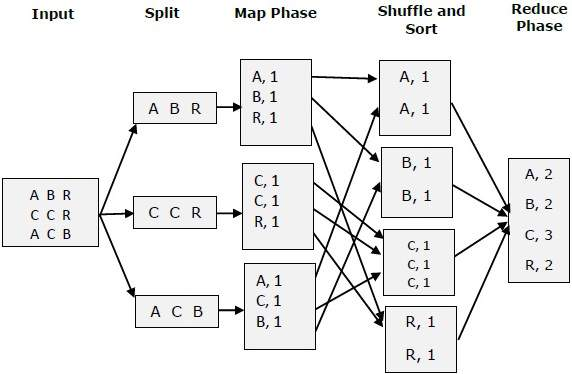
\includegraphics[width=0.9\textwidth]{./MapReduce.jpg}
\end{center}
\end{frame}

\begin{frame}[label={sec:org2494477},fragile]{MapReduce}
 \begin{itemize}
\item \texttt{@distributed} nos va a permitir indicar una función de reducción al estilo MapReduce.
\item La función de reducción tomará los elementos reducidos hasta ahora y un nuevo elemento. Deberá de funcionar sin importar el orden que apliquemos.
\item Con la función de reducción podemos combinar los datos de cada chunk.
\end{itemize}
\end{frame}

\begin{frame}[label={sec:orgf6ddc54},fragile]{MapReduce}
 \begin{verbatim}
A = rand(1000)

x = Distributed.@distributed (+) for i in 1:length(A)
      sqrt(A[i])
    end
\end{verbatim}
\end{frame}

\begin{frame}[label={sec:orgb64f3e1},fragile]{RemoteChannel}
 \begin{itemize}
\item De forma similar a \texttt{Channel}, vamos a encontrar un sistema de comunicación entre nodos de alto nivel llamado \texttt{RemoteChannel}.
\item Cada \texttt{RemoteChannel} tiene que vivir en un nodo.
\item Podemos configurar el Channel interno a través de una función.
\end{itemize}
\end{frame}

\begin{frame}[label={sec:orgbf1dddb},fragile]{RemoteChannel}
 \begin{verbatim}
@everywhere function suma(data_ch, sum_ch)
    c = 0.0
    a = take!(data_ch)
    for x in a
        c = c + x
    end
    put!(sum_ch, c)
end
\end{verbatim}
\end{frame}

\begin{frame}[label={sec:org78e8e06},fragile]{RemoteChannel}
 \begin{verbatim}
data_ch = RemoteChannel(()->Channel{Any}(4))
sum_ch = RemoteChannel(()->Channel{Float64}(4))
for w in Distributed.workers()
    @spawnat w suma(data_ch, sum_ch)
end
chunks = Iterators.partition(
    a, length(a) ÷ Distributed.nworkers())
for chunk in chunks
    put!(data_ch, chunk)
end
s = 0.0
for i in 1:Distributed.nworkers()
    s += take!(sum_ch)
end
\end{verbatim}
\end{frame}

\begin{frame}[label={sec:org34117cb}]{Dagger}
\begin{itemize}
\item Nos hemos centrado principalmente en datos con un flujo muy sencillo.
\item ¿Qué pasa cuando el flujo de datos se entrelaza y se complica?
\item Puede que no identifiquemos manualmente los momentos para paralelizar.
\item Hay librerías como \emph{Dagger} que construyen un grafo dirigido acíclico de las operaciones sobre nuestro código.
\begin{itemize}
\item Y paralelizan cuando es posible, tanto por recursos como porque tenemos todos los datos para empezar
\end{itemize}
\end{itemize}
\end{frame}

\begin{frame}[label={sec:org1829179},fragile]{Dagger}
 \begin{verbatim}
a = Dagger.@spawn rand(100, 100)
b = Dagger.@spawn rand(100, 100)
# a y b se ejecutan en paralelo

c = Dagger.@spawn a + b 
d = Dagger.@spawn a * b
# c y d se ejecutan en paralelo
wait(Dagger.@spawn println("sum: ", c, ", prod: ", d))
\end{verbatim}
\end{frame}
\end{document}
